\chapter{Machine Learning}
\label{chap:three}
\section{Terminology}
\section{Algorithms}
\subsection{Logistic Regression}
\subsection{Decision Tree}
\subsection{Logistic Regression}
\subsection{Naive Bayes}
\subsection{K-Nearest Neighbors}
\subsection{Random Forest}
\subsection{Gradient Boosting}
\subsection{Support Vector Machine}
\subsection{Neural Networks}
\section{Evaluation Metrics}
\subsection{Confusion Matrix}


\begin{equation}\label{eq}
C = {c_{i,j} = \sum_{l=1}^{m}[(y_l=i) \land (f(x_l)=j)]}
\end{equation}

\begin{equation}\label{eq}
    C_{i \times j} = \begin{bmatrix}
    c_{1,1} & c_{2,1} & \cdots & c_{1,j} \\
    c_{2,1} & c_{2,2} & \cdots & c_{2,j} \\
    \vdots & \vdots & \ddots & \vdots \\
    c_{i,1} & c_{i,2} & \cdots & c_{i,j} \\
    \end{bmatrix}
\end{equation}


\begin{equation}
    C_{2 \times 2} = \begin{bmatrix}
    TP & FN \\
    FP & TN \\
    \end{bmatrix}
    \end{equation}


\subsection{Accuracy}

\begin{equation}\label{eq}
    Accuracy = \frac{TP + FN}{TP + TN + FP + FN}
\end{equation}

\subsection{Recall}

\begin{equation}\label{eq}
    Precision = \frac{TP}{TP + FN}
\end{equation}

\subsection{Precision}

\begin{equation}\label{eq}
    Precision = \frac{TP}{TP + FP}
\end{equation}

\subsection{F1 Score}

\begin{equation}\label{eq}
    F1 = \frac{2 \times Precision \times Recall}{Precision + Recall} = \frac{2 \times TP}{2 \times TP + FP + FN}
\end{equation}

\subsection{AUC}

\begin{equation}\label{eq}
    AUC = \int_{0}^{1} TPR \left(FPR^{-1}\left(x \right)\right) dx
\end{equation}

\subsection{Kolmogorov-Smirnov}

\begin{equation}\label{eq}
    KS = \max_{x \in \mathbb{R}} \left| \hat{F}_n \left(x \right) - F \left(x \right) \right|
\end{equation}


\subsection{Somer's D}

\begin{equation}\label{eq}
    SD = \frac{\tau \left(X, Y\right)}{\sqrt{\tau \left(X, X\right) \tau \left(Y, Y\right)}}
\end{equation}


\subsection{Matthews Correlation Coefficient}

\begin{equation}\label{eq}
    MCC = \frac{TP \times TN - FP \times FN}{\sqrt{(TP + FP) (TP + FN) (TN + FP) (TN + FN)}}
\end{equation}


\subsection{Brier Score Loss}

\begin{equation}\label{eq}
    BSL = \frac{1}{n} \sum_{i=1}^{n} (y_i - \hat{y}_i)^2
\end{equation}


\subsection{Jaccard Score}


\begin{equation}\label{eq}
    JC = \frac{|y \cap \hat{y} |}{|y \cup \hat{y} |}
    \end{equation}


\subsection{Zero-One Loss}

\begin{equation}\label{eq}
    ZOL = \frac{1}{n} \sum_{i}^{n} \delta_{y_{i=1} \neq \hat{y}_{i}} \text{ , where } \delta_{y_{i} \neq \hat{y}_{i}} = \begin{cases}
        1, & \text{if $x<0$}.\\
        0, & \text{otherwise}.
      \end{cases}
\end{equation}
\section{Hyperparameter Tuning}

dfgdfgf

\subsection{Grid Search}
\subsection{Random Search}
\subsection{Bayesian Optimization}
\section{Imbalanced Class Distribution}
\subsection{Random Oversampling}
\subsection{SMOTE Oversampling}
\subsection{ADASYN Oversampling}

dfgdfgf

\label{sec:citace}

Text text text text text text text text text text text text text text text. Text text text text text text text text text text. Text text text text text text text text text text text text text text text. Text text  \citet{Haufler2006}.

Text text text text text text text text text text text text text text text. Text text text text text text text \cite[see, \latinfont{inter alia},][pg.~10]{Haaparanta1996}. 

\section{Special Czech, Slovak, and German letters}

\r{u}, \'{a}, \v{s}, \v{d}, \v{t}, \v{r}, \^{o}, \ss{}, \"{o}

\section{Acronyms}

Text text text text text text text text text text text text text text text. Text text text text text text text text text text. Text text text text text text. Politicians usualy like inward \ac{FDI} and an \ac{MNC} appreciates \ac{FDI} subsidies. Are \acp{MNC} greedy?

\section{Figures}

To achieve compatibility with PDF/A 2u, your file must not include links to external fonts, audio, video, or scripts. On the other hand, your file must declare each color environment you use, it must include all the pictures/figures either in jpeg or PDF/A 2u format, used fonts compliant under Unicode (your file cannot use any external fonts), and it must include meta-data in XMP format.


Most troubleshooting comes from the conversion of figures to compliant formats. You can convert from simple PDF using Adobe Acrobat:
\begin{itemize}
	\item Select File >> Save as Other >> Archivable PDF (PDF/A)
				\begin{figure}[!h]
					\centering
						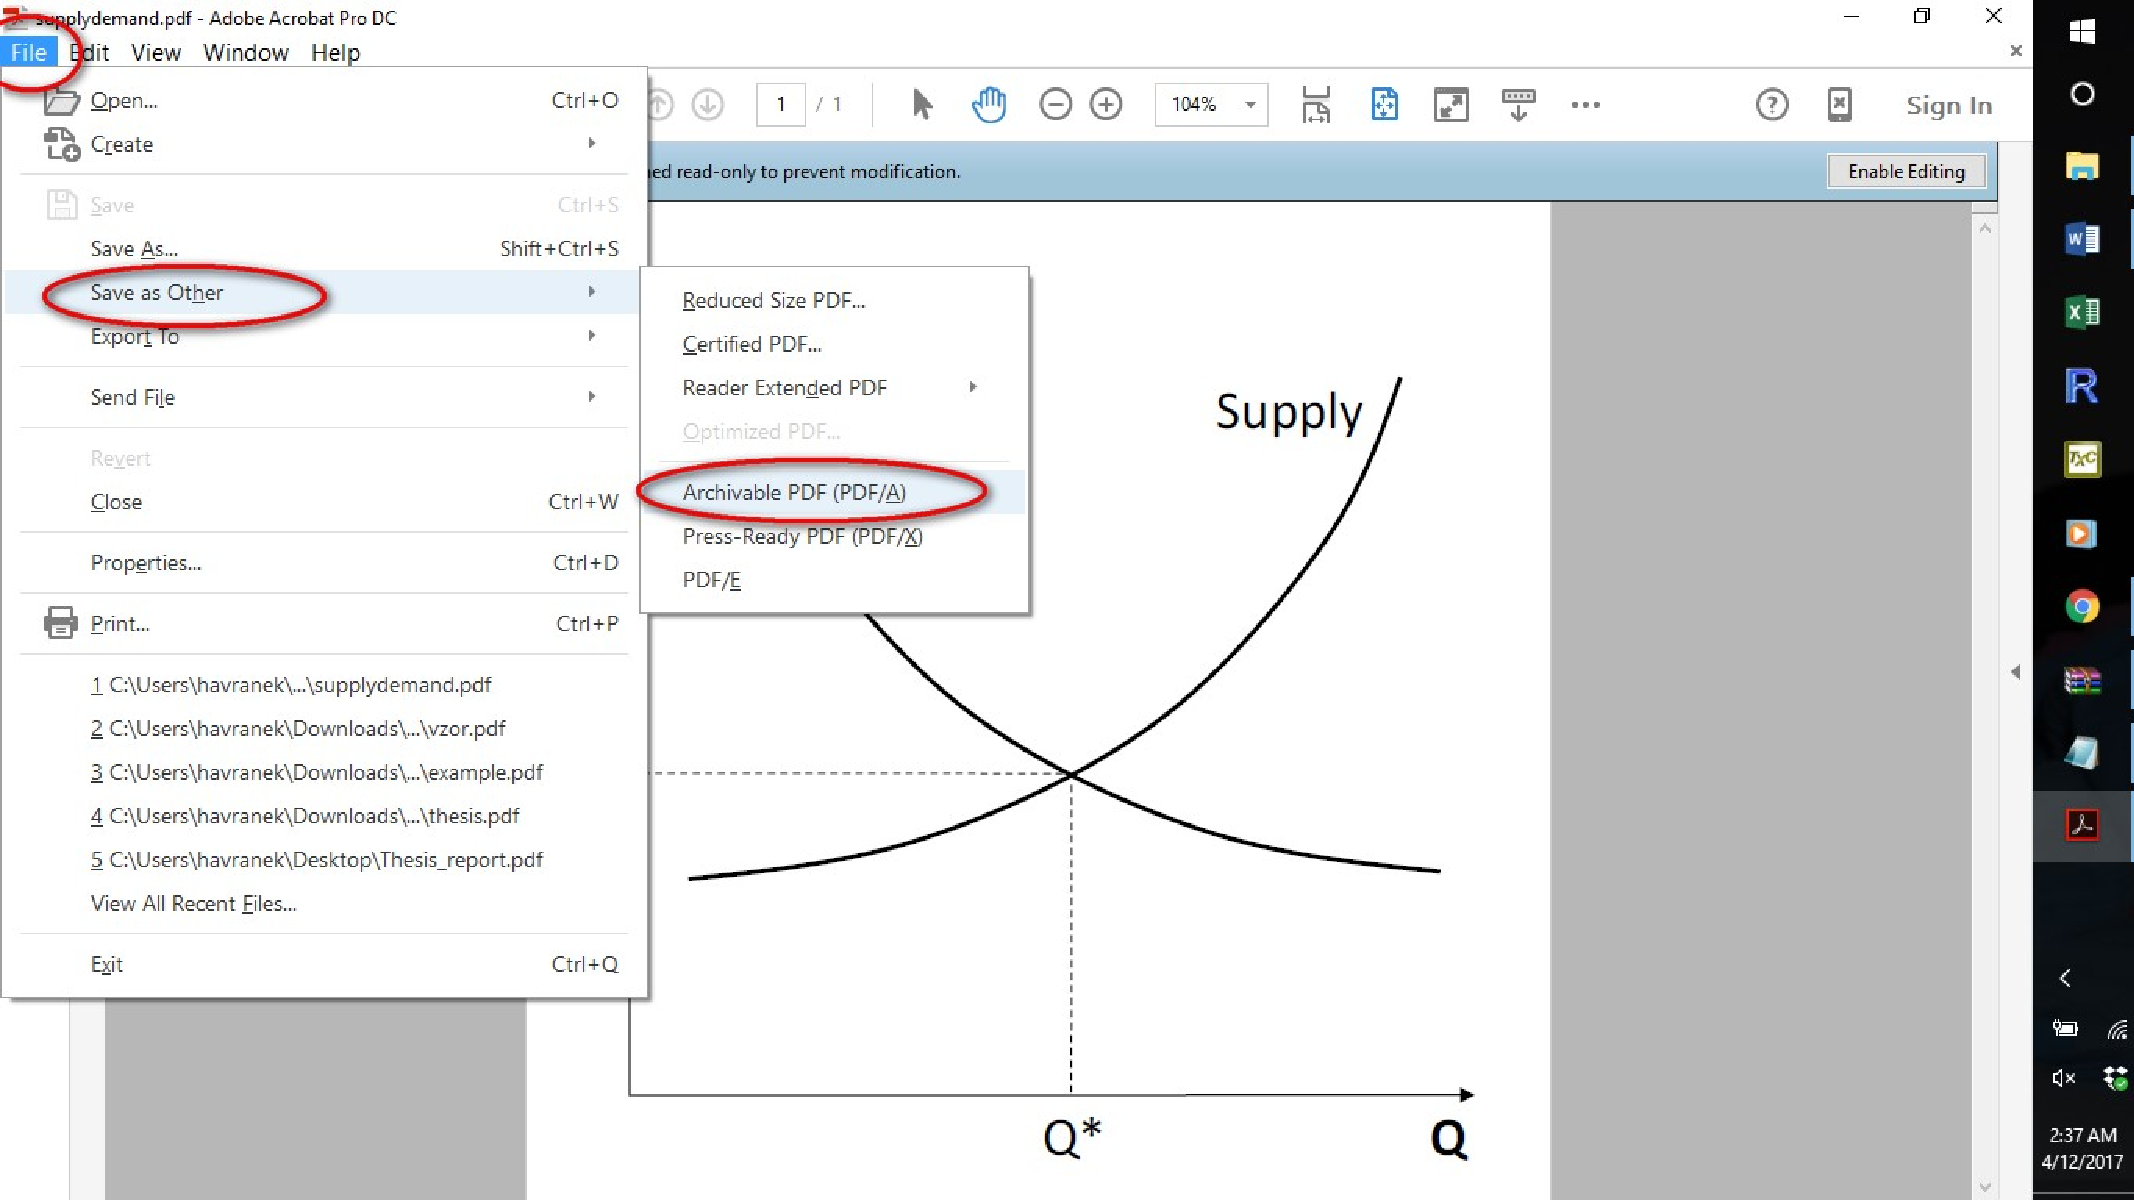
\includegraphics[width=0.6\textwidth]{Figures/conversion1.pdf}
					\label{fig:conversion1}
				\end{figure}
	\item Save as PDF/A-2u:
			\begin{figure}[!h]
				\centering
					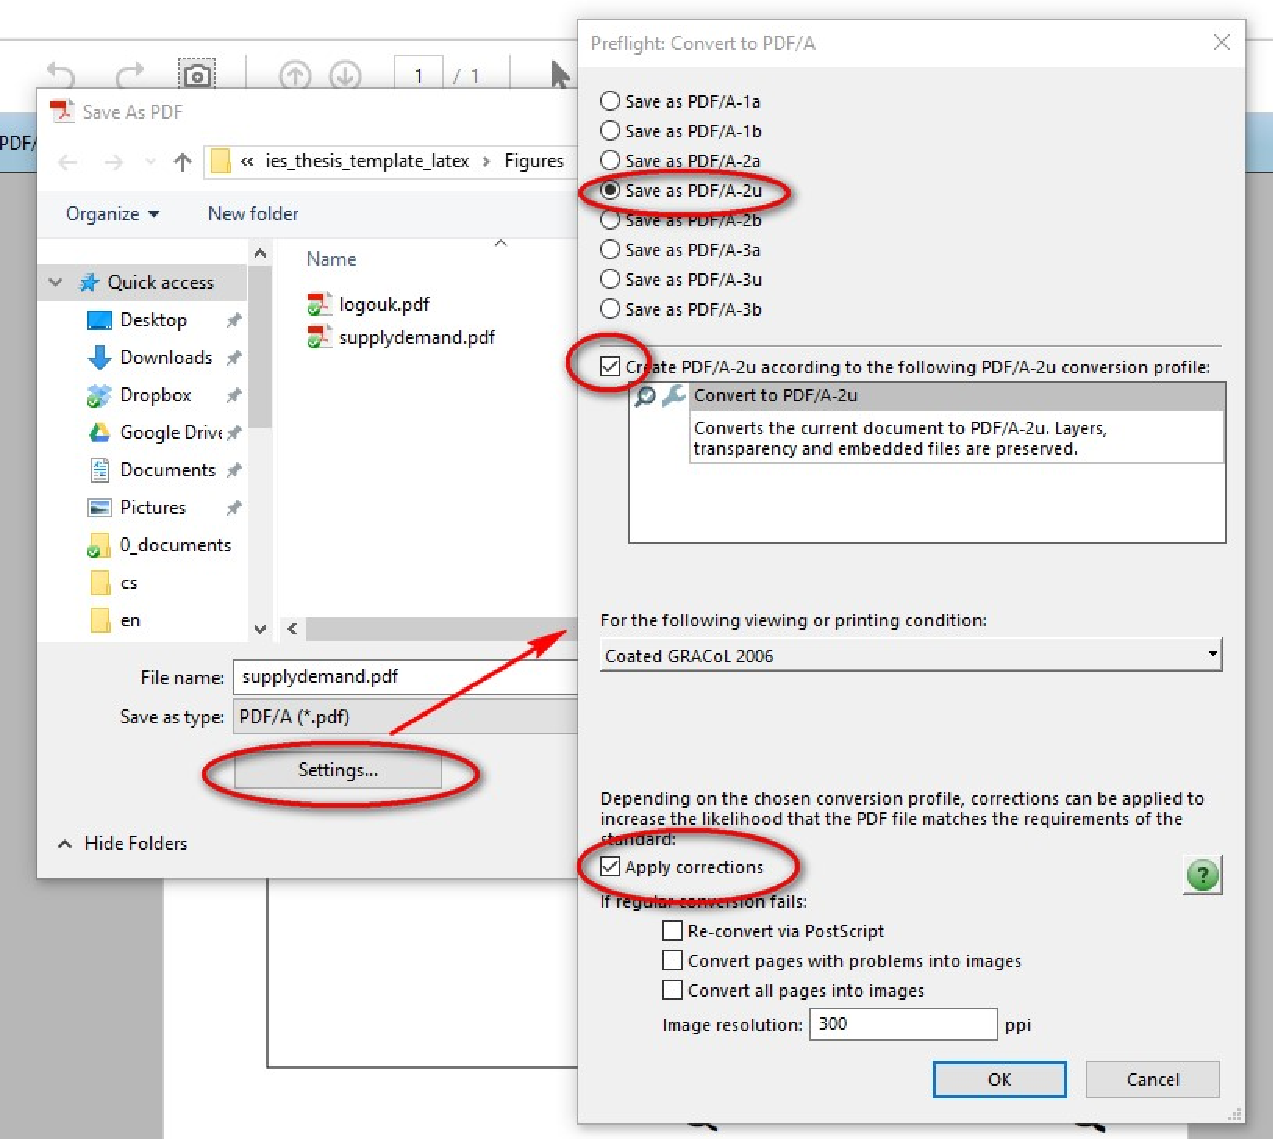
\includegraphics[width=0.6\textwidth]{Figures/conversion2.pdf}
				\label{fig:conversion2}
			\end{figure}
\end{itemize}	


But most of the vector graphics gets distorted to lower quality in Adobe (like pictures in pdfs generated from Stata, unless jpeg is sufficient for you). You can also use GhostScript, the conversion tool is provided by courtesy of the Faculty of Mathematics and Physics at

\vspace{0.5cm}
\textbf{\href{https://kam.mff.cuni.cz/pdfix/}{https://kam.mff.cuni.cz/pdfix/}}
\vspace{0.5cm}

Text text text text text text.\footnote{Text text text text text text text text text text text text text text text. Text text text text text text text text text text. Text text text text text text.} Font of Latin phrases should be consistent: Furthermore, there is no \latinfont{ex post} price effect, all things being equal (\latinfont{ceteris paribus}). This is \latinfont{per se} truth.

\begin{figure}[!htbp]
\begin{center}
\caption{Market equilibrium}
\label{fig:supply}
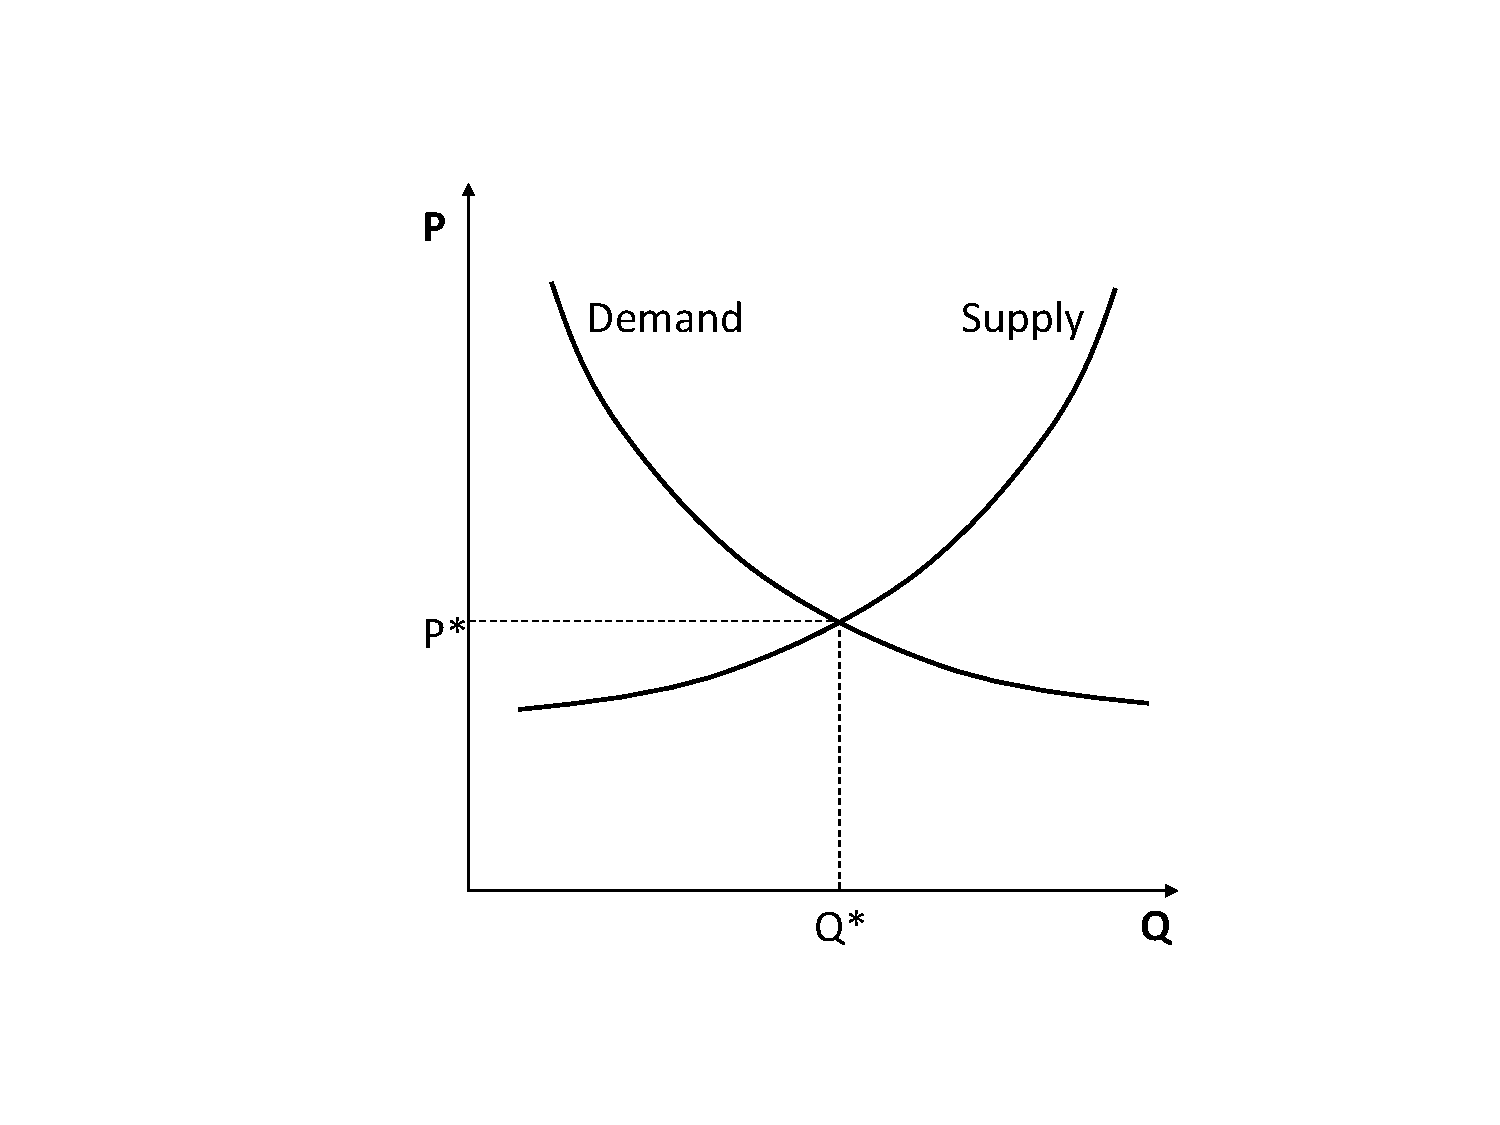
\includegraphics[width=60mm]{Figures/supplydemand}
\end{center}\vspace{-0.5cm}
\begin{source}\cite{Haufler2006}.\end{source}
\end{figure}

Look at the \autoref{fig:supply}. Text text text text text text text text text text. Text text text text text text. Text text text text text text text text text text. Text text text text text text text text text text.



\section{Tables}

If you use Stata, you might want to check the \texttt{sutex}, \texttt{outtable}, \texttt{outtex}, and \texttt{estout} tools, which help you with exporting Stata tables to \LaTeX{}.

\begin{table}[!htbp]
\begin{center}
	\caption[Calibration table]{Model's predictions}\label{tab:values}
\begin{tabular}{lrrrrrrrrrr}
\toprule
\textit{Case} &        $Y_1$ &        $Y_2$ &  $\tau_1$ &  $\tau_2$ &          $a$ &          $n$\\
\midrule
CR---Slovakia &       10.9 &         10 &       0.24 &       0.19 &          1,000 &       2.16\\

CR---Poland &       13.3 &         12 &       0.24 &       0.19 &          1,000 &       0.38\\

CR---Hungary &       10.4 &          8 &       0.24 &       0.16 &          1,000 &        1.10\\
\bottomrule
\end{tabular}  
\end{center}
\begin{source} If the source is author himself (like a calculation output), this line is redundant.\end{source}
\end{table}

Text text text text text text text text text text text text text text text. Text text text text text text text text text text. Text text text text text text. Text text text text text text text text text text. Text text text text text text text text text text.

\section{Boxes}

Text text text text text text text text text text text text text text text. Text text text text text text text text text text. Text text text text text text. Text text text text text text text text text text. Text text text text text text text text text text. Let us make a box:

\begin{figure}[!htbp]
\begin{center}
\caption{Boxy's example}\label{box:values}
\begin{boxeditemize}
	\item Welcome to Boxy paragraph. 
We sincerely hope you will
all enjoy the show.
	\item
Welcome to Boxy paragraph.
We sincerely hope you will
all enjoy the show.
	\item 
Welcome to Boxy paragraph.
We sincerely hope you will
all enjoy the show.
\end{boxeditemize}
\end{center}
\begin{source}\cite{Haaparanta1996}\end{source}
\end{figure}

Text text text text text text text text text text text text text text text. Text text text text text text text text text text. Text text text text text text. Text text text text text text text text text text. Text text text text text text text text text text.

\section{Theorems, Definitions, \ldots}

\begin{defin}[My original definition]\label{de:definice1}
This is a definition.
\end{defin}

\begin{ass}[My realistic assumption]\label{as:predpoklad1}
This is an assumption.
\end{ass}

\begin{prop}[My clever proposition]\label{pr:veta1}
This is a proposition.
\end{prop}

\begin{lemma}[My useful lemma]\label{le:lemma1}
This is a lemma.
\end{lemma}

\begin{exam}\label{ex:priklad1}
This is an example.
\end{exam}

\begin{proof}
This is a proof.
\end{proof}

\section{Equations}
\label{rovnice}

\subsection{Nonumbered Equations}

Text text text text text text text text text text text text text text text. Text text text text text text text text text text. Text text text text text text. Text text text text text text text text text text. Text text text text text text text text text text.

    \[ U = \underbrace{\int_0^{\infty} \frac{1}{1-\sigma}\left(C^{1-\sigma} -1 \right) e^{-\rho t} \ud t}_\text{meaning of life} \]

\subsection{Numbered Equations}

Text text text text text text text text text text text text text text text. Text text text text text text text text text text. Text text text text text text. Text text text text text text text text text text. Text text text text text text text text text text.
\begin{equation}\label{eq:rovnice1}
    U = \int_0^{\infty} \overbrace{ \frac{1}{1-\sigma}\left(C^{1-\sigma} -1 \right)}^\text{instantaneous utility} e^{-\rho t} \ud t
\end{equation}

\subsection{Matrix Equations}

Text text text text text text text text text text text text text text text. Text text text text text text text text text text. Text text text text text text. Text text text text text text text text text text. Text text text text text text text text text text.

\begin{equation}\label{eq:rovnice2}
    \mat{A} = \mat{B} + \mat{C}
\end{equation}

\section{Cross-references}

\begin{itemize}
    \item to literature~\citep[pg.~10]{Bjorvatn2006} 	
            or~\citet[pg.~10]{Haufler2006},
    \item to~\autoref{fig:supply},														%or use \autoref
    \item see~\autoref{tab:values},
    \item to~\autoref{rovnice},
    \item to~\defref{de:definice1}, to~\proref{pr:veta1},
            \exaref{ex:priklad1}, 
    \item to equations like this: see~\eqref{eq:rovnice1}.
\end{itemize}

\section{Source codes}

You can input a source code like this:
\begin{matlab}{.9\linewidth}{dgreen}
    omega = 1;
    syms zeta;
    jmn = [1 2*zeta*omega omega^2];
    figure(1);
        for zeta = 1E-5 : 0.2 : 1+1E-12
            G = tf(omega^2,subs([1 2*zeta*omega omega^2]));
            bode(G); hold on;
        end
    legend('\zeta = 0','\zeta = 0,2','\zeta = 0,4','\zeta = 0,6',');
\end{matlab}
Should you prefer a different font size, redefine file \texttt{Styles/Mystyle.sty}.



\section{Paragraphs}

Usually you should not use the first person singular (I) in your text, write we instead. As a general recommendation, use the first person sparsely, sometimes it can be replaced by a phrase like ``This work presents \ldots.''

Text text text text text text text text text text text text text text text. Text text text text text text text text text text. Text text text text text text. Text text text text text text text text text text. Text text text text text text text text text text. Text text text text text text \citep{Haufler2006}. Let us make two paragraphs:

\paragraph{Proin} Text text text text text text text text text text text text text text text. Text text text text text text text text text text. Text text text text text text. Text text text text text text text text text text. Text text text text text text text text text text.
Text text text text text text text text text text text text text text text. Text text text text text text text text text text. Text text text text text text. And a subparagraph:
\subparagraph{Velit} Text text text text text text text text text text text text text text text. Text text text text text text text text text text. Text text text text text text. Text text text text text text text text text text. Text text text text text text text text text text.


